\let\raggedright\relax%

\documentclass[10pt, xcolor={svgnames}]{beamer}

% package.
\usepackage[utf8]{inputenc}
\usetheme[]{Boadilla}
\usecolortheme{dolphin}
\usepackage{amssymb,amsmath,amsfonts, amscd, wasysym}
\usepackage{pifont}% http://ctan.org/pkg/pifont
\usepackage{etoolbox}
\usepackage[T1]{fontenc}
\usepackage{graphicx}
\usepackage{stmaryrd}
\usepackage{verbatim}
\usepackage[normalem]{ulem}
\usepackage{tikz}
\usepackage{xcolor}
\usepackage{xspace}
\usefonttheme{professionalfonts}
\usetikzlibrary{patterns}
\usetikzlibrary{calc}
\usetikzlibrary{shadows.blur}


\usepackage{algorithmicx}
\usepackage{algpseudocode}

\definecolor{antiquewhite}{rgb}{1, 0.98, 0.96}

\setbeamercolor{background canvas}{bg=antiquewhite}

\definecolor{ballblue}{rgb}{0.13, 0.67, 0.8}
\colorlet{newballblue}{ballblue!80!black}


\newcommand{\vect}[1]{\textbf{#1}}
\newcommand{\piv}{\color{red}{\bullet}}
\newcommand{\bul}{\small{\bullet}}
\newcommand{\cand}{\color{blue}{\bullet}}
\newcommand{\lib}[1]{\textcolor{SlateBlue}{\textsf{#1}}\xspace}
\newcommand{\refer}[1]{\textcolor{DarkCyan}{[#1]}}
\newcommand{\kwrd}[1]{\textcolor{newballblue}{#1}}
\newcommand{\calB}{\ensuremath{\mathcal{B}}}
\newcommand{\calA}{\ensuremath{\mathcal{A}}}
\newcommand{\calC}{\ensuremath{\mathcal{C}}}
\newcommand{\calO}{\ensuremath{\mathcal{O}}}
\newcommand{\calT}{\ensuremath{\mathcal{T}}}
\newcommand{\bigO}[1]{\ensuremath{\mathcal{O}\left( #1 \right)} }
\newcommand{\bigOtilde}[1]{\ensuremath{\tilde{\mathcal{O}}\left( #1 \right)} }
\newcommand{\xor}{\ensuremath{\oplus}}
\newcommand{\ZZ}{\mathbb{Z}}
\newcommand{\FF}{\ensuremath{\mathbb{F}}}
\newcommand{\EE}{\ensuremath{\mathbb{E}}}
\newcommand{\RR}{\ensuremath{\mathbb{R}}}
\newcommand{\round}[1]{\ensuremath{\lfloor #1 \rceil}}
\newcommand{\fround}[1]{\ensuremath{\lfloor #1 \rfloor}}
\newcommand{\calV}{\ensuremath{\mathcal{V}}}
\newcommand{\green}[1]{\textcolor{ForestGreen}{#1}}
\newcommand{\linbox}{\lib{LinBox}}
\newcommand{\ps}[2]{\langle #1,#2 \rangle}
\renewcommand{\vec}{\mathbf}

\newcommand{\quizz}[3]{\only<#1>{\phantom{#3}}\only<#2->{\alert{#3}}}

\newcommand{\Ucolor}{\color{LimeGreen}}
\newcommand{\Lcolor}{\color{cyan}}
%\newcommand{\Acolor}{\color{Gray}}
\newcommand{\Scolor}{\color{SlateBlue}}
\newcommand{\Acolortext}{\textcolor{Gray}}
\newcommand{\Scolortext}{\textcolor{SlateBlue}}
\newcommand{\Ucolortext}{\textcolor{LimeGreen}}
\newcommand{\Lcolortext}{\textcolor{DeepSkyBlue}}
\newcommand{\scol}[1]{\textcolor{Red}{#1}}


\newcommand{\sspcs}{\texttt{SS-PCS}}
\newcommand{\sspcsIV}{\ensuremath{\texttt{SS-PCS}_4}}





\definecolor{bluegray}{rgb}{0.4, 0.6, 0.8}
\definecolor{seagreen}{rgb}{0.18, 0.55, 0.34}

\definecolor{amethyst}{rgb}{0.6, 0.4, 0.8}
\definecolor{darkred}{rgb}{0.5, 0.0, 0.13}
\definecolor{bondiblue}{rgb}{0.0, 0.58, 0.71}
\newcommand{\kcol}[1]{\textcolor{newballblue}{#1}}

\newcommand{\veca}{\kcol{\vec a}}

\newcommand{\red}{\alert}

%\addtobeamertemplate{navigation symbols}{}{%
%    \usebeamerfont{footline}%
%    \usebeamercolor[fg]{footline}%
%    \hspace{1em}%
%    \insertframenumber/\inserttotalframenumber
%}
\renewcommand\footnoterule{{\color{white}\hrule height 0.5pt width \paperwidth}}

%\makeatother
%\setbeamertemplate{footline}{%
%  \leavevmode%
%\textcolor{white}{\hrule}
%  \footnoterule
%  \hbox{%
%  \begin{beamercolorbox}[wd=\paperwidth,ht=0.25in,dp=1ex,right]{footlinecolor}
%    \hfill \hfill
%    \insertframenumber{} \hspace*{.5cm}
%    \vskip0pt 
%  \end{beamercolorbox}}%
%  \vskip0pt}

\beamertemplatenavigationsymbolsempty

\makeatletter
\colorlet{beamer@blendedblue}{green!10!blue!75}
\makeatother



\setbeamercolor*{block title example}{bg=pink!55!cyan!40!white, fg=cyan!50!green!80!gray}
%\AtBeginEnvironment{blockexample}{\setbeamercolor{itemize item}{fg=cyan!50!black}}
\setbeamercolor{example text}{fg=green!50!black}

%\setbeamercolor*{block title}{bg=Cyan!30!blue!15!white, fg=green!10!blue!75}
%\AtBeginEnvironment{block}{\setbeamercolor{itemize item}{fg=green!10!blue!75}}
%\setbeamercolor{block text}{fg=cyan!80!}

\newenvironment{algoblock}[1]{%
	\setbeamercolor{block title}{bg=SkyBlue!80!white, fg=cyan!70!black}
	%\setbeamercolor{block body}{bg=Green}
	\begin{block}{#1}}{\end{block}
}


\newcommand{\mybibentry}[4]{\item[\small{\refer{#1}}]\small{ \kwrd{#2}}\\ \item[]\footnotesize{\textit{#3} (#4)}}

\newcommand{\cmark}{\ding{51}}%
\newcommand{\xmark}{\ding{55}}%

\usetikzlibrary{patterns}
\usetikzlibrary{snakes}
\usetikzlibrary{arrows}
\usetikzlibrary{backgrounds}
\usetikzlibrary{shapes}
\usetikzlibrary{shadows}
\usetikzlibrary{calc}
\usetikzlibrary{decorations}
\usetikzlibrary{decorations.pathmorphing}
\usetikzlibrary{decorations.shapes}
\usetikzlibrary{decorations.markings}
\usetikzlibrary{positioning}


\newcommand{\tikzmat}[2] {
\draw[thick] let \p1 = (#1 |- #2),
                 \p2 = (#2 |- #1) in
   ($ (#1) + (0.05,-0.1) $) -- ++(-0.15, 0)  -- ($ (\p1) + (-0.1,0.1) $) -- ++(0.15,0)
   ($ (\p2) + (-0.05,-0.1) $) -- ++(0.15, 0) -- ($ (#2) + (0.1,0.1) $) -- ++(-0.15,0);
}




\newcommand{\tcancel}[2][black]{%
\begin{tikzpicture}
\node[draw=#1,cross out,inner sep=1pt] (a){#2};
\end{tikzpicture}%
}

\pgfdeclarepatternformonly{my crosshatch dots}{\pgfqpoint{-2pt}{-2pt}}{\pgfqpoint{10pt}{10pt}}{\pgfqpoint{12pt}{12pt}}%
{
    \pgfpathcircle{\pgfqpoint{0pt}{0pt}}{.5pt}
    \pgfpathcircle{\pgfqpoint{6pt}{6pt}}{.5pt}
    \pgfusepath{fill}
}


\setbeamertemplate{footline}{%
	% \leavevmode%
	%\textcolor{white}{\hrule}
	%  \footnoterule
	\hbox{%
		\begin{beamercolorbox}[wd=\paperwidth,ht=0.25in,dp=1ex,right]{footlinecolor}
			\hfill \hfill
			\insertframenumber{} \hspace*{.5cm}
			\vskip0pt 
	\end{beamercolorbox}}%
	% \vskip0pt
}



\title[IN100 Cours 4]{\textbf{Fondements informatiques I}\\
Cours 5: Types mutables et immutables\\ Fonctions (suite et fin)}

\author[]{Sorina Ionica \texttt{sorina.ionica@uvsq.fr} \\~\\Sandrine Vial  \texttt{sandrine.vial@uvsq.fr} }


\institute{}

\date{}


%\setbeamercolor{normal text}{fg=black}

\begin{document}


\begin{frame}
\titlepage
\end{frame}



\begin{frame}[fragile]{Types mutables et immutables}

\vspace{1 cm}
En Python, on distingue deux types d'objets: 
\vspace{0.5 cm}
\begin{enumerate}
\item[1.] objets immutables : qu'on ne peut pas changer
   \begin{itemize}
   \item entiers, flottants
   \item tuples
   \item chaînes de caractères
\end{itemize}
\end{enumerate}
\begin{columns}
\column{6cm}
\vspace*{-2 cm}
\begin{exampleblock}{}
\begin{verbatim}
x=3
x+=1
\end{verbatim}
\end{exampleblock}
\column{4 cm}

\vspace{1 cm}
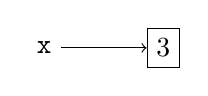
\begin{tikzpicture}
% Variable name (node)
\node (var) at (0,0) {\texttt{x}};
% Rectangle (node)
\node[draw, rectangle, minimum height=0.5cm, right=1cm] (rect) at (0.3,0) {3};
% Arrow from variable to rectangle
\draw[->] (var) -- (rect);
\end{tikzpicture}


\vspace{0.7 cm}
\pause
Après incrémentation: 

\vspace{0.3 cm}
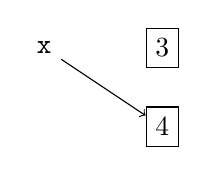
\begin{tikzpicture}
% Variable name (node)
\node (var) at (0,0) {\texttt{x}};
% Rectangle (node)
\node[draw, rectangle, minimum height=0.5cm] (rect) at (1.5,0) {3};
\node[draw, rectangle, minimum height=0.5cm] (rect1) at (1.5,-1) {4};
% Arrow from variable to rectangle
\draw[->] (var) -- (rect1);
\end{tikzpicture}
\end{columns}
\end{frame}



\begin{frame}[fragile]{Variables mutables et immutables}

\begin{enumerate}
\item[2.] objets mutables: dont on peut modifier le contenu
\begin{itemize}
\item les listes
\item les ensembles (sets)
\item les dictionnaires (qu'on verra plus tard)
\end{itemize}
\end{enumerate}

\vspace{2 cm}
\begin{columns}
\column{5 cm}
\vspace{-1.5 cm}

\begin{exampleblock}{}
\begin{verbatim}
liste=[1,2,3]
liste[0]=5
\end{verbatim}
\end{exampleblock}
\column{4 cm}
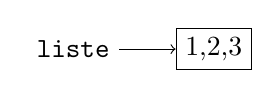
\begin{tikzpicture}
% Variable name (node)
\node (var) at (0,0) {\texttt{liste}};
% Rectangle (node)
\node[draw, rectangle, minimum height=0.5cm, right=1cm] (rect) at (0.3,0) {1,2,3};
% Arrow from variable to rectangle
\draw[->] (var) -- (rect);
\end{tikzpicture}

\vspace{1 cm}
\pause

Après modification: 

\vspace{0.5 cm}
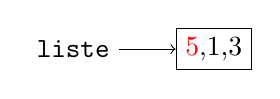
\begin{tikzpicture}
% Variable name (node)
\node (var) at (0,0) {\texttt{liste}};
% Rectangle (node)
\node[draw, rectangle, minimum height=0.5cm, right=1cm] (rect) at (0.3,0) {\textcolor{red}{5},1,3};
% Arrow from variable to rectangle
\draw[->] (var) -- (rect);
\end{tikzpicture}
\end{columns}
\end{frame}


\begin{frame}[fragile]{Questions}


Que se passe-t-il à l'exécution? 

\begin{exampleblock}{}
\begin{verbatim}
mon_tuple=(1,2,3)
mon_tuple[0]=5
\end{verbatim}
\end{exampleblock}


\begin{exampleblock}{}
\begin{verbatim}
chaine="hello world"
chaine[0]='H'
\end{verbatim}
\end{exampleblock}

\end{frame}

\begin{frame}[fragile]{Questions}

Ecrivez un programme qui prend une chaîne de caractères et affiche la chaîne avec la première lettre de chaque mot en majuscule. 

\pause
\begin{exampleblock}{}
\small{
\begin{verbatim}
resultat=""
debut_mot = True  # Indique si on est au début d’un mot

for c in chaine:
        if debut_mot and c != " ":      # Si c'est le début d'un mot
            resultat += c.upper()       # Mettre en majuscule
            debut_mot = False
        else:
            resultat += c                     
        if c == " ":                   
            debut_mot = True

print(resultat)
\end{verbatim}
}
\end{exampleblock}




\end{frame}


\begin{frame}[fragile]{Les variables d'une fonction}

\begin{itemize}
\item   Les variables définies dans une fonction sont appelées \textbf{variables
locales}.
\item La portée d'une variable locale est limitée à la fonction où elle a été
définie, on ne peut pas y faire référence en dehors.
\end{itemize}


\vspace{0.5 cm}

\begin{exampleblock}{Exemple}
\begin{verbatim}
def incremente(x):
    x +=  1
    z = 2

incremente(2)
print(x) 
#print(z) 
\end{verbatim}
\end{exampleblock}

\vspace{0.5 cm}

Lors de l'exécution,  l'affichage produit un NameError (variable pas définie). 
\end{frame}



\begin{frame}[fragile]{\'Evaluation de la fonction}

\begin{itemize}
\item Les arguments sont des variables locales à la fonction.
\item Les arguments sont passés par la copie d'une référence sur l'objet
  donné en argument.
%\item Le corps de la fonction est évalué comme un code normal et la fonction
%se termine soit à la fin du bloc de code indenté, soit quand une
 % instruction \texttt{return} est atteinte
%\item la fonction peut appeler une autre fonction ou elle-même (récursivité)
\end{itemize}

\vspace{1 cm}

\begin{columns}
\column{6 cm}
\begin{exampleblock}{}
\begin{verbatim}
def incremente(x):
    x += 1
    
y = 0
incremente(y)
print(y)
\end{verbatim}
\end{exampleblock}

\column{4 cm}
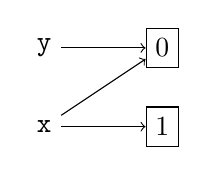
\begin{tikzpicture}
% Variable name (node)
\onslide<2->
\node[draw, rectangle, minimum height=0.5cm] (rect) at (1.5,0) {0};
\node (var) at (0,0) {\texttt{y}};
\draw[->] (var) -- (rect);

\onslide<3->
\node (var1) at (0,-1) {\texttt{x}};

% Rectangle (node)
% Arrow from variable to rectangle
\only<3>
\draw[->] (var1) -- (rect);
\onslide<4->
\node[draw, rectangle, minimum height=0.5cm] (rect1) at (1.5,-1) {1};
\draw[->] (var1) -- (rect1);
\end{tikzpicture}
\end{columns}

\end{frame}



\begin{frame}[fragile]{Référence sur une liste}


\textbf{\`A retenir :}

\begin{itemize}
\item Sur une liste, on peut modifier son contenu depuis la fonction, car objet mutable. 
\end{itemize}

\vspace{1 cm}

\begin{columns}
\column{6 cm}

\begin{exampleblock}{}
\begin{verbatim}
def incrementeListe(k):
    for i in range(len(k)):
        k[i] += 1

l = [3,4,5]
incrementeListe(l)
print(l)
\end{verbatim}
\end{exampleblock}
\column{5 cm}
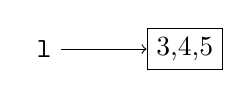
\begin{tikzpicture}
% Variable name (node)
\node (var) at (0,0) {\texttt{l}};
% Rectangle (node)
\node[draw, rectangle, minimum height=0.5cm, right=1cm] (rect) at (0.3,0) {3,4,5};
% Arrow from variable to rectangle
\draw[->] (var) -- (rect);
\end{tikzpicture}

\pause
\vspace{1 cm}
Après appel \texttt{incrementeListe}

\vspace{0.3 cm}

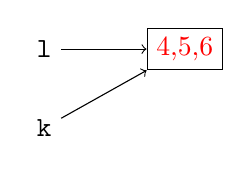
\begin{tikzpicture}
% Variable name (node)
\node (var) at (0,0) {\texttt{l}};
\node (var1) at (0,-1) {\texttt{k}};

% Rectangle (node)
\node[draw, rectangle, minimum height=0.5cm, right=1cm] (rect) at (0.3,0) {\textcolor{red}{4,5,6}};
% Arrow from variable to rectangle
\draw[->] (var) -- (rect);
\draw[->] (var1) -- (rect);
\end{tikzpicture}


\end{columns}



  
\end{frame}



\begin{frame}[fragile]{Référence sur une liste}

\textbf{\`A retenir :}
\begin{itemize}
\item Cependant, on ne peut pas modifier la liste elle même! 
\end{itemize}

\vspace{0.5 cm}


\begin{columns}
\column{5 cm}
\begin{exampleblock}{}
\begin{verbatim}
def supprimeListe(k):
    k= []

l = [3,4,5]
supprimeListe(l)
print(l)
\end{verbatim}		
\end{exampleblock}
\column{4 cm}
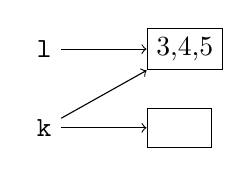
\begin{tikzpicture}
% Variable name (node)
\node (var) at (0,0) {\texttt{l}};
\node[draw, rectangle, minimum height=0.5cm, right=1cm] (rect) at (0.3,0) {3,4,5};
\draw[->] (var) -- (rect);

\onslide<2->
\node (var1) at (0,-1) {\texttt{k}};
% Rectangle (node)
% Arrow from variable to rectangle
\only<2>
\draw[->] (var1) -- (rect);
\onslide<3->
\node<3->[draw, rectangle, minimum height=0.5cm, right=1cm] (rect1) at (0.3,-1) {~~~~~~};
\draw[->] (var1) -- (rect1);
\end{tikzpicture}
\end{columns}

\end{frame}


\begin{frame}[fragile]{Utilisation de variables globales}

\small{
\begin{itemize}
\item Les variables définies hors des fonctions sont \textbf{globales} par
opposition aux variables \textbf{locales} des fonctions. 
   \item On peut les utiliser dans toutes les fonctions.
\item \textcolor{red}{Attention:}  on ne peut pas changer la valeur d'une variable globale à l'intérieur d'une
fonction. 
\end{itemize}
}
\begin{exampleblock}{}
\small{
\begin{verbatim}
x = 1
print(x)

def affiche(): #utilisation d'une variable globale
    print(x)
    
x += 3
affiche()

def ajoute(): #modification d'une variable globale
    x += 1
    
ajoute()
print(x)    
\end{verbatim}
}
\end{exampleblock}

\end{frame}


\begin{frame}[fragile]{Utilisation de variables globales}

\begin{itemize}

\item Pour modifier une variable globale, il faut spécifier dans la fonction que la variable est globale
par le mot clé \texttt{global}.
\begin{itemize}
\item Il est \emph{déconseillé} de faire usage de ce mot clé et des variables
globales en général.
\end{itemize}
\end{itemize}


\begin{exampleblock}{}
\begin{verbatim}
x=1

def ajoute(): #modif. d'une var. globale avec le mot clé "global"
    global x
    x += 1
   
ajoute()
print(x)
\end{verbatim}
\end{exampleblock}
\end{frame}


\begin{frame}[fragile]{Utilisation de variables globales}

Qu'affiche-t-on à l'exécution? 


\begin{exampleblock}{}
\begin{verbatim}
x=3

def ajoute():  #rédefinir une variable globale
    x=5
    x += 1
   
ajoute()
print(x)
\end{verbatim}
\end{exampleblock}

\vspace{0.5 cm}

Explication : On a rédefinit la variable \texttt{x}. 
\end{frame}

\begin{frame}[fragile]{Représentation des arguments dans un appel de
fonction}

\begin{itemize}
\item On peut donner des valeurs par défaut aux arguments d'une fonction de la
manière suivante: \\
\texttt{def\ ma\_fonction(pays,\ age\ =\ 1,\ nom\ =\ "toto")}.

\item Les variables ayant une valeur par défaut peuvent être omises.
\end{itemize}


\begin{exampleblock}{}

\begin{verbatim}
def ma_fonction(pays, age = 1, nom = "toto"):
    print(nom," a ", age, "ans et vit en ", pays)
    
ma_fonction("france")
ma_fonction("allemagne", 18, "kurt")
ma_fonction("italie", 77)
\end{verbatim}
\end{exampleblock}

\end{frame}

\frame[containsverbatim]{\frametitle{Ordre des arguments dans un appel de
fonction}

\begin{itemize}
\item En règle générale, on respecte l'ordre des arguments donnes dans la signature. 
\item On peut également donner les arguments dans le désordre en spécifiant leur nom.
\end{itemize}

\vspace{0.5 cm}

\begin{exampleblock}{Exemple}
\begin{verbatim}
def ma_fonction(pays, age = 1, nom = "toto"):
    print(nom," a ", age, "ans et vit en ", pays)
    
ma_fonction(nom = "kader", age = 18, pays = "algérie")
ma_fonction("france", nom = "sylvie")    
\end{verbatim}
\end{exampleblock}

}


\frame[containsverbatim]{\frametitle{Appel de fonction depuis une autre fonction}

La fonction peut appeler une autre fonction. %ou elle-même (récursivité). 

\begin{exampleblock}{Exemple}
\begin{verbatim} 
def doubler(x):
    return 2*x
    
def sommer(x,y):
    return x+doubler(y)
    
print(sommer(2,3))
\end{verbatim}

\end{exampleblock}

}

\frame[containsverbatim]{\frametitle{Appel de fonction depuis une autre fonction}

Que affiche-t-on à l'exécution?  Au besoin, corriger afin de doubler les valeurs dans la liste. 

\begin{exampleblock}{}
\begin{verbatim} 
def doubler(x):
    return 2*x
    
 
 def doubler_liste(l):
      for i in range(len(l)):
          doubler(l[i])
      return l		   

l=[2,3,4]		   
print(doubler_liste(l))
\end{verbatim}
\end{exampleblock}

}


\begin{frame}[fragile]{Expressions lambda}

\vspace{1 cm}

\begin{itemize}
\item Pour définir une fonction courte, il existe une syntaxe alternative
utilisant l'opérateur \textbf{lambda}.

\item La définition doit tenir sur une ligne. 
\begin{itemize}
\item On ne peut pas utiliser des instructions de contrôle
\end{itemize}
\end{itemize}

\begin{exampleblock}{}
\begin{verbatim} 
g = lambda x: x*2  
print(g(2))
\end{verbatim}
\end{exampleblock}

\vspace{0.5 cm}
\pause

\begin{itemize}
\item La fonction définie par un lambda est anonyme, c'est à dire qu'elle n'a pas de nom.
\begin{itemize}
\item C'est utile quand la fonction sert une seule fois %, par exemple comme argument d'une autre fonction.
\end{itemize}
\end{itemize}

\begin{exampleblock}{}
\begin{verbatim} 
print((lambda x: x*2)(3))

#applique la fonction à chaque élément de range(10)
list(map(lambda x: x*2,range(10)))
\end{verbatim}
\end{exampleblock}

\end{frame}




\end{document}



